\documentclass{article}\usepackage[]{graphicx}\usepackage[]{color}
%% maxwidth is the original width if it is less than linewidth
%% otherwise use linewidth (to make sure the graphics do not exceed the margin)
\makeatletter
\def\maxwidth{ %
  \ifdim\Gin@nat@width>\linewidth
    \linewidth
  \else
    \Gin@nat@width
  \fi
}
\makeatother

\definecolor{fgcolor}{rgb}{0.345, 0.345, 0.345}
\newcommand{\hlnum}[1]{\textcolor[rgb]{0.686,0.059,0.569}{#1}}%
\newcommand{\hlstr}[1]{\textcolor[rgb]{0.192,0.494,0.8}{#1}}%
\newcommand{\hlcom}[1]{\textcolor[rgb]{0.678,0.584,0.686}{\textit{#1}}}%
\newcommand{\hlopt}[1]{\textcolor[rgb]{0,0,0}{#1}}%
\newcommand{\hlstd}[1]{\textcolor[rgb]{0.345,0.345,0.345}{#1}}%
\newcommand{\hlkwa}[1]{\textcolor[rgb]{0.161,0.373,0.58}{\textbf{#1}}}%
\newcommand{\hlkwb}[1]{\textcolor[rgb]{0.69,0.353,0.396}{#1}}%
\newcommand{\hlkwc}[1]{\textcolor[rgb]{0.333,0.667,0.333}{#1}}%
\newcommand{\hlkwd}[1]{\textcolor[rgb]{0.737,0.353,0.396}{\textbf{#1}}}%
\let\hlipl\hlkwb

\usepackage{framed}
\makeatletter
\newenvironment{kframe}{%
 \def\at@end@of@kframe{}%
 \ifinner\ifhmode%
  \def\at@end@of@kframe{\end{minipage}}%
  \begin{minipage}{\columnwidth}%
 \fi\fi%
 \def\FrameCommand##1{\hskip\@totalleftmargin \hskip-\fboxsep
 \colorbox{shadecolor}{##1}\hskip-\fboxsep
     % There is no \\@totalrightmargin, so:
     \hskip-\linewidth \hskip-\@totalleftmargin \hskip\columnwidth}%
 \MakeFramed {\advance\hsize-\width
   \@totalleftmargin\z@ \linewidth\hsize
   \@setminipage}}%
 {\par\unskip\endMakeFramed%
 \at@end@of@kframe}
\makeatother

\definecolor{shadecolor}{rgb}{.97, .97, .97}
\definecolor{messagecolor}{rgb}{0, 0, 0}
\definecolor{warningcolor}{rgb}{1, 0, 1}
\definecolor{errorcolor}{rgb}{1, 0, 0}
\newenvironment{knitrout}{}{} % an empty environment to be redefined in TeX

\usepackage{alltt}
\usepackage{standalone}
\standalonetrue
\ifstandalone
  \usepackage{../../../haziq_article}
  \addbibresource{../../../bib/library.bib}
\fi





\IfFileExists{upquote.sty}{\usepackage{upquote}}{}
\begin{document}

\subsection{Iris data set}

\begin{knitrout}\small
\definecolor{shadecolor}{rgb}{0.969, 0.969, 0.969}\color{fgcolor}

{\centering 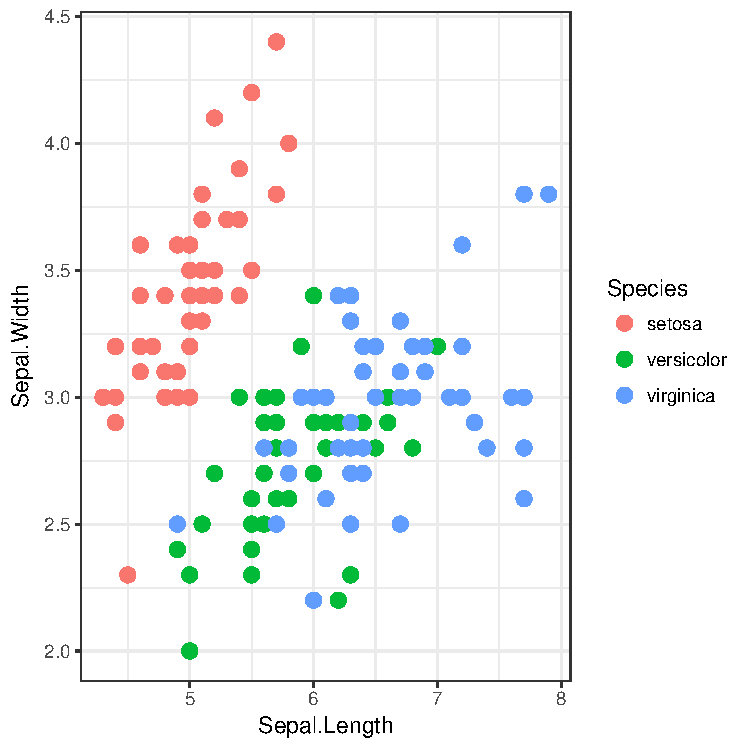
\includegraphics[width=6cm,height=6cm]{figure/iris_data-1} 
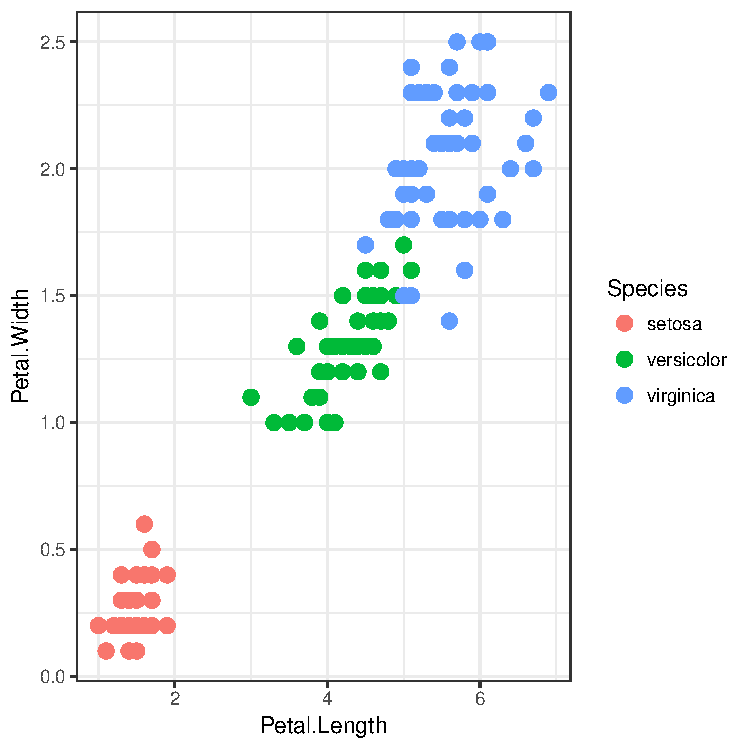
\includegraphics[width=6cm,height=6cm]{figure/iris_data-2} 
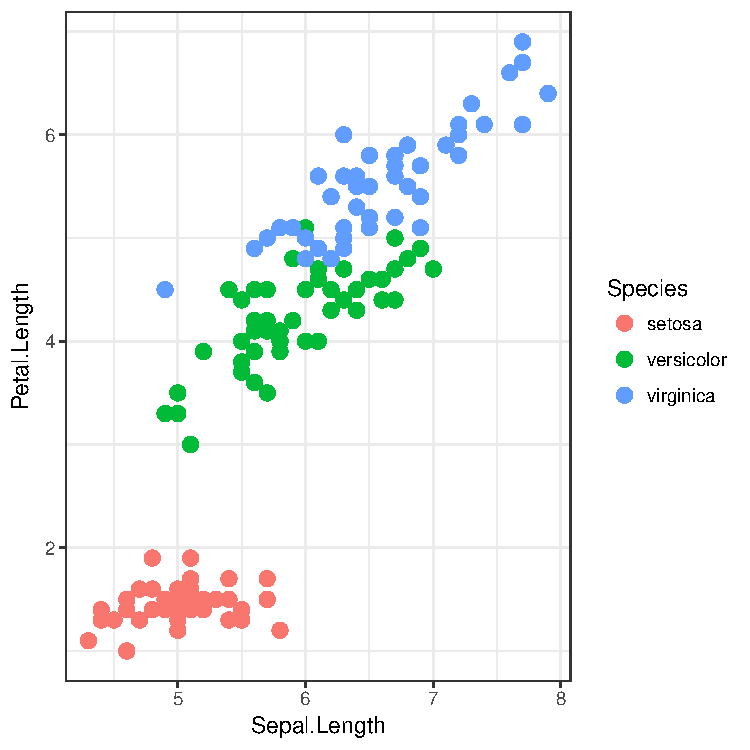
\includegraphics[width=6cm,height=6cm]{figure/iris_data-3} 
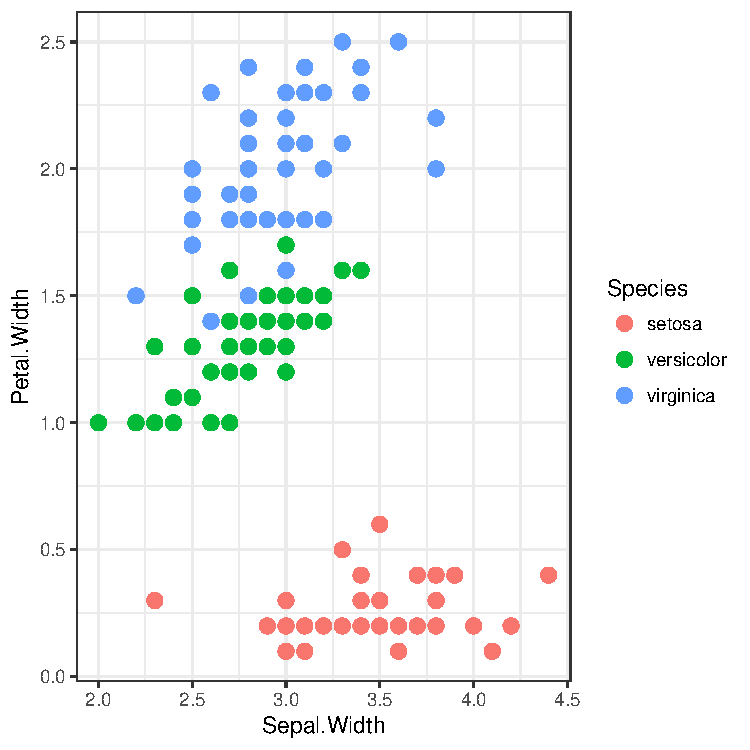
\includegraphics[width=6cm,height=6cm]{figure/iris_data-4} 
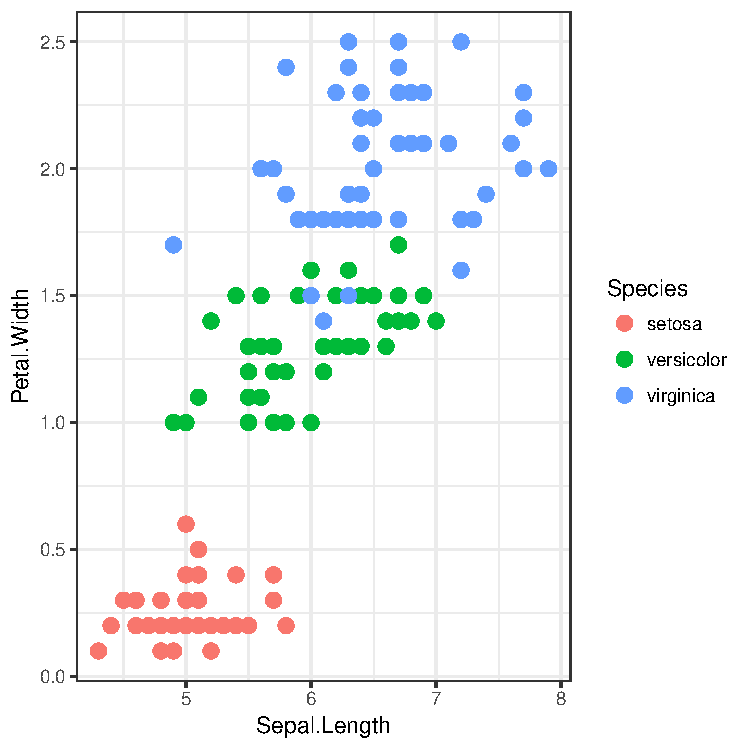
\includegraphics[width=6cm,height=6cm]{figure/iris_data-5} 
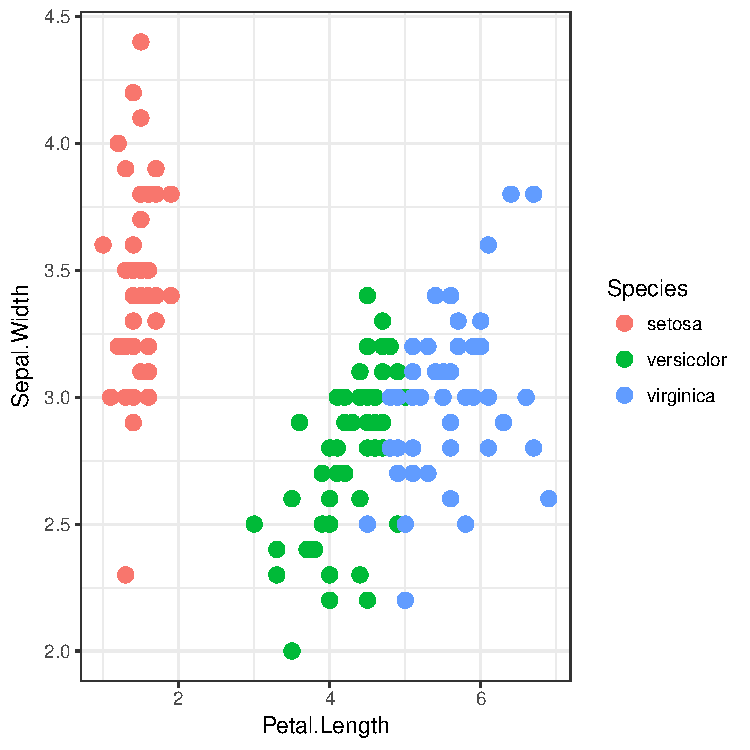
\includegraphics[width=6cm,height=6cm]{figure/iris_data-6} 

}



\end{knitrout}

\begin{knitrout}\small
\definecolor{shadecolor}{rgb}{0.969, 0.969, 0.969}\color{fgcolor}\begin{kframe}
\begin{alltt}
\hlstd{R> }\hlstd{(mod} \hlkwb{<-} \hlkwd{iprobit_mult}\hlstd{(y, X,} \hlkwc{silent} \hlstd{=} \hlnum{TRUE}\hlstd{))}
\end{alltt}
\begin{verbatim}
## Lower bound value =  -55.60715 
## Iterations =  100 
## 
##           Class = 1 Class = 2 Class = 3
## Intercept  -0.21708   1.20009  -1.13551
## lambda     -0.35226  -0.35226  -0.35226
\end{verbatim}
\begin{alltt}
\hlstd{R> }\hlkwd{plot}\hlstd{(mod)}
\end{alltt}
\end{kframe}

{\centering 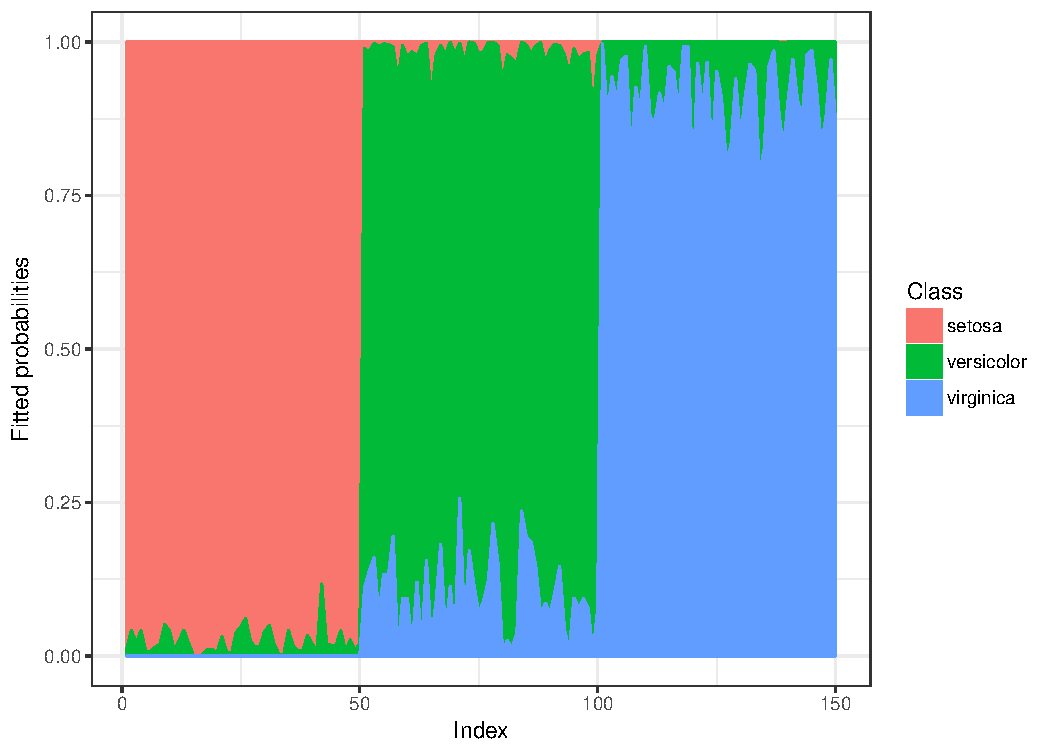
\includegraphics[width=\maxwidth]{figure/iris_mod-1} 

}


\begin{kframe}\begin{alltt}
\hlstd{R> }\hlkwd{iplot_lb}\hlstd{(mod)}
\end{alltt}
\end{kframe}

{\centering 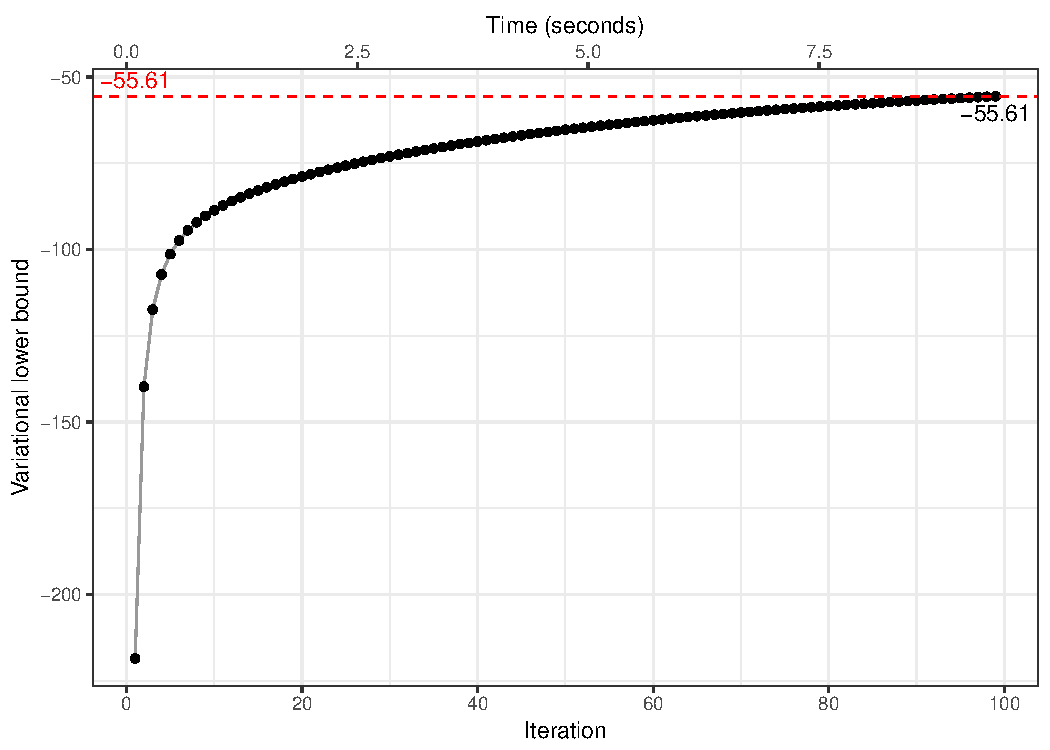
\includegraphics[width=\maxwidth]{figure/iris_mod-2} 

}



\end{knitrout}

\subsection{Vowel recognition data set}

\begin{knitrout}\small
\definecolor{shadecolor}{rgb}{0.969, 0.969, 0.969}\color{fgcolor}\begin{kframe}
\begin{verbatim}
##   class    x.1   x.2    x.3   x.4    x.5   x.6    x.7    x.8    x.9   x.10
## 1     1 -3.639 0.418 -0.670 1.779 -0.168 1.627 -0.388  0.529 -0.874 -0.814
## 2     2 -3.327 0.496 -0.694 1.365 -0.265 1.933 -0.363  0.510 -0.621 -0.488
## 3     3 -2.120 0.894 -1.576 0.147 -0.707 1.559 -0.579  0.676 -0.809 -0.049
## 4     4 -2.287 1.809 -1.498 1.012 -1.053 1.060 -0.567  0.235 -0.091 -0.795
## 5     5 -2.598 1.938 -0.846 1.062 -1.633 0.764  0.394 -0.150  0.277 -0.396
## 6     6 -2.852 1.914 -0.755 0.825 -1.588 0.855  0.217 -0.246  0.238 -0.365
\end{verbatim}
\end{kframe}
\end{knitrout}
\begin{knitrout}\small
\definecolor{shadecolor}{rgb}{0.969, 0.969, 0.969}\color{fgcolor}\begin{kframe}
\begin{alltt}
\hlstd{R> }\hlkwd{set.seed}\hlstd{(}\hlnum{123}\hlstd{)}
\hlstd{R> }\hlstd{(mod} \hlkwb{<-} \hlkwd{iprobit_mult}\hlstd{(vow.tr}\hlopt{$}\hlstd{class, vow.tr[,} \hlopt{-}\hlnum{1}\hlstd{],} \hlkwc{kernel} \hlstd{=} \hlstr{"FBM"}\hlstd{,} \hlkwc{silent} \hlstd{=} \hlnum{TRUE}\hlstd{))}
\end{alltt}
\begin{verbatim}
## Lower bound value =  -736.8918 
## Iterations =  100 
## 
##           Class = 1 Class = 2 Class = 3 Class = 4 Class = 5 Class = 6
## Intercept  -0.11514   0.13838   0.04304   0.07129   0.21767   0.46536
## lambda     -0.13430  -0.13430  -0.13430  -0.13430  -0.13430  -0.13430
##           Class = 7 Class = 8 Class = 9 Class = 10 Class = 11
## Intercept   0.40117   -0.3387   0.47458   -0.06605    0.67874
## lambda     -0.13430   -0.1343  -0.13430   -0.13430   -0.13430
\end{verbatim}
\begin{alltt}
\hlstd{R> }\hlkwd{plot}\hlstd{(mod)}
\end{alltt}
\end{kframe}

{\centering 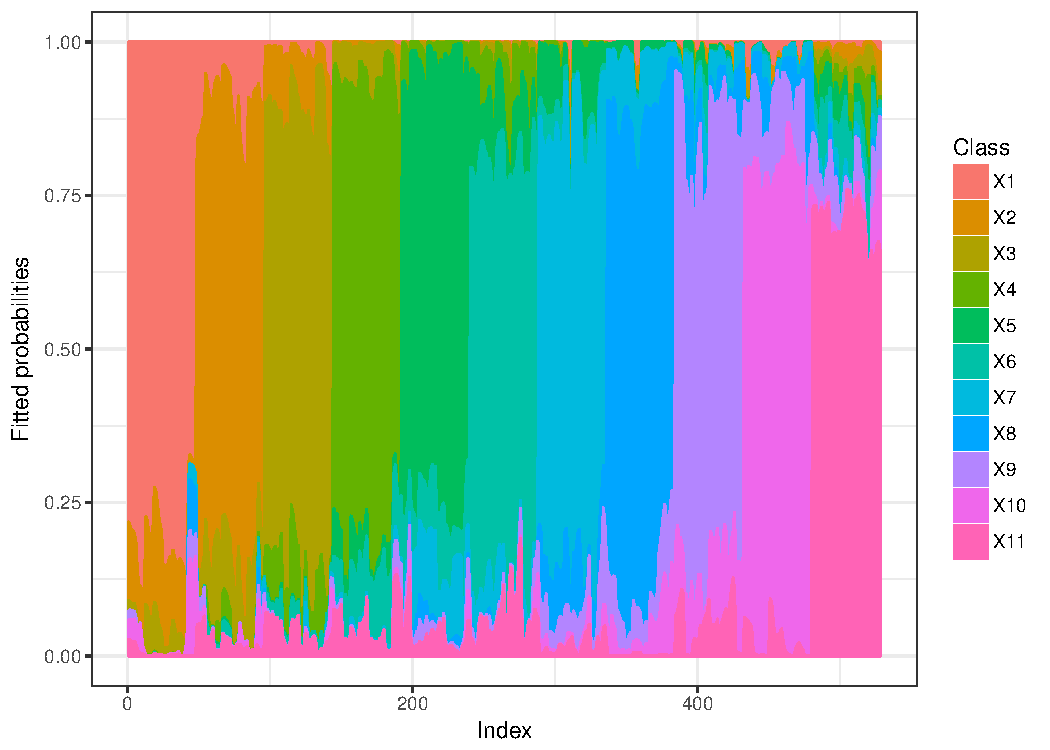
\includegraphics[width=\maxwidth]{figure/vowel_mod-1} 

}


\begin{kframe}\begin{alltt}
\hlstd{R> }\hlkwd{predict}\hlstd{(mod,} \hlkwc{X.test} \hlstd{= vow.ts[,} \hlopt{-}\hlnum{1}\hlstd{],} \hlkwc{y.test} \hlstd{= vow.ts[,} \hlnum{1}\hlstd{])}
\end{alltt}
\begin{verbatim}
## Test error rate: 41 %
\end{verbatim}
\end{kframe}
\end{knitrout}
\begin{table}[!h]
\centering
\begin{tabular}{lrr}
\toprule
\multicolumn{1}{c}{ } & \multicolumn{2}{c}{Error rates} \\ \cmidrule(l{2pt}r{2pt}){2-3}
  & Training & Test\\
\midrule
k-Nearest neighbours & NA & 44\\
Linear regression & 48 & 67\\
Linear discriminant analysis & 32 & 56\\
Neural network & NA & 45\\
FDA/BRUTO & 6 & 44\\
\addlinespace
FDA/MARS & 13 & 39\\
I-probit (FBM-0.5) & 0 & 41\\
\bottomrule
\end{tabular}
\end{table}



\end{document}


